\section{Implementation}
\label{sec:implementation}

While our proposed API is general and not language specific, we have implemented
\sysname{} prototype in Rust (\textasciitilde 4000 lines of code). \sysname{} is
open source on GitHub.\footnote{URL elided for anonymity.}  Applications use
\sysname{} as a library and configure the execution mode---profiling, runtime as
client, or runtime as server---with command line arguments.  We have implemented
the deployment manager that can start, stop, and update clients/servers as shell
scripts.

% \begin{figure}
%   \centering
%   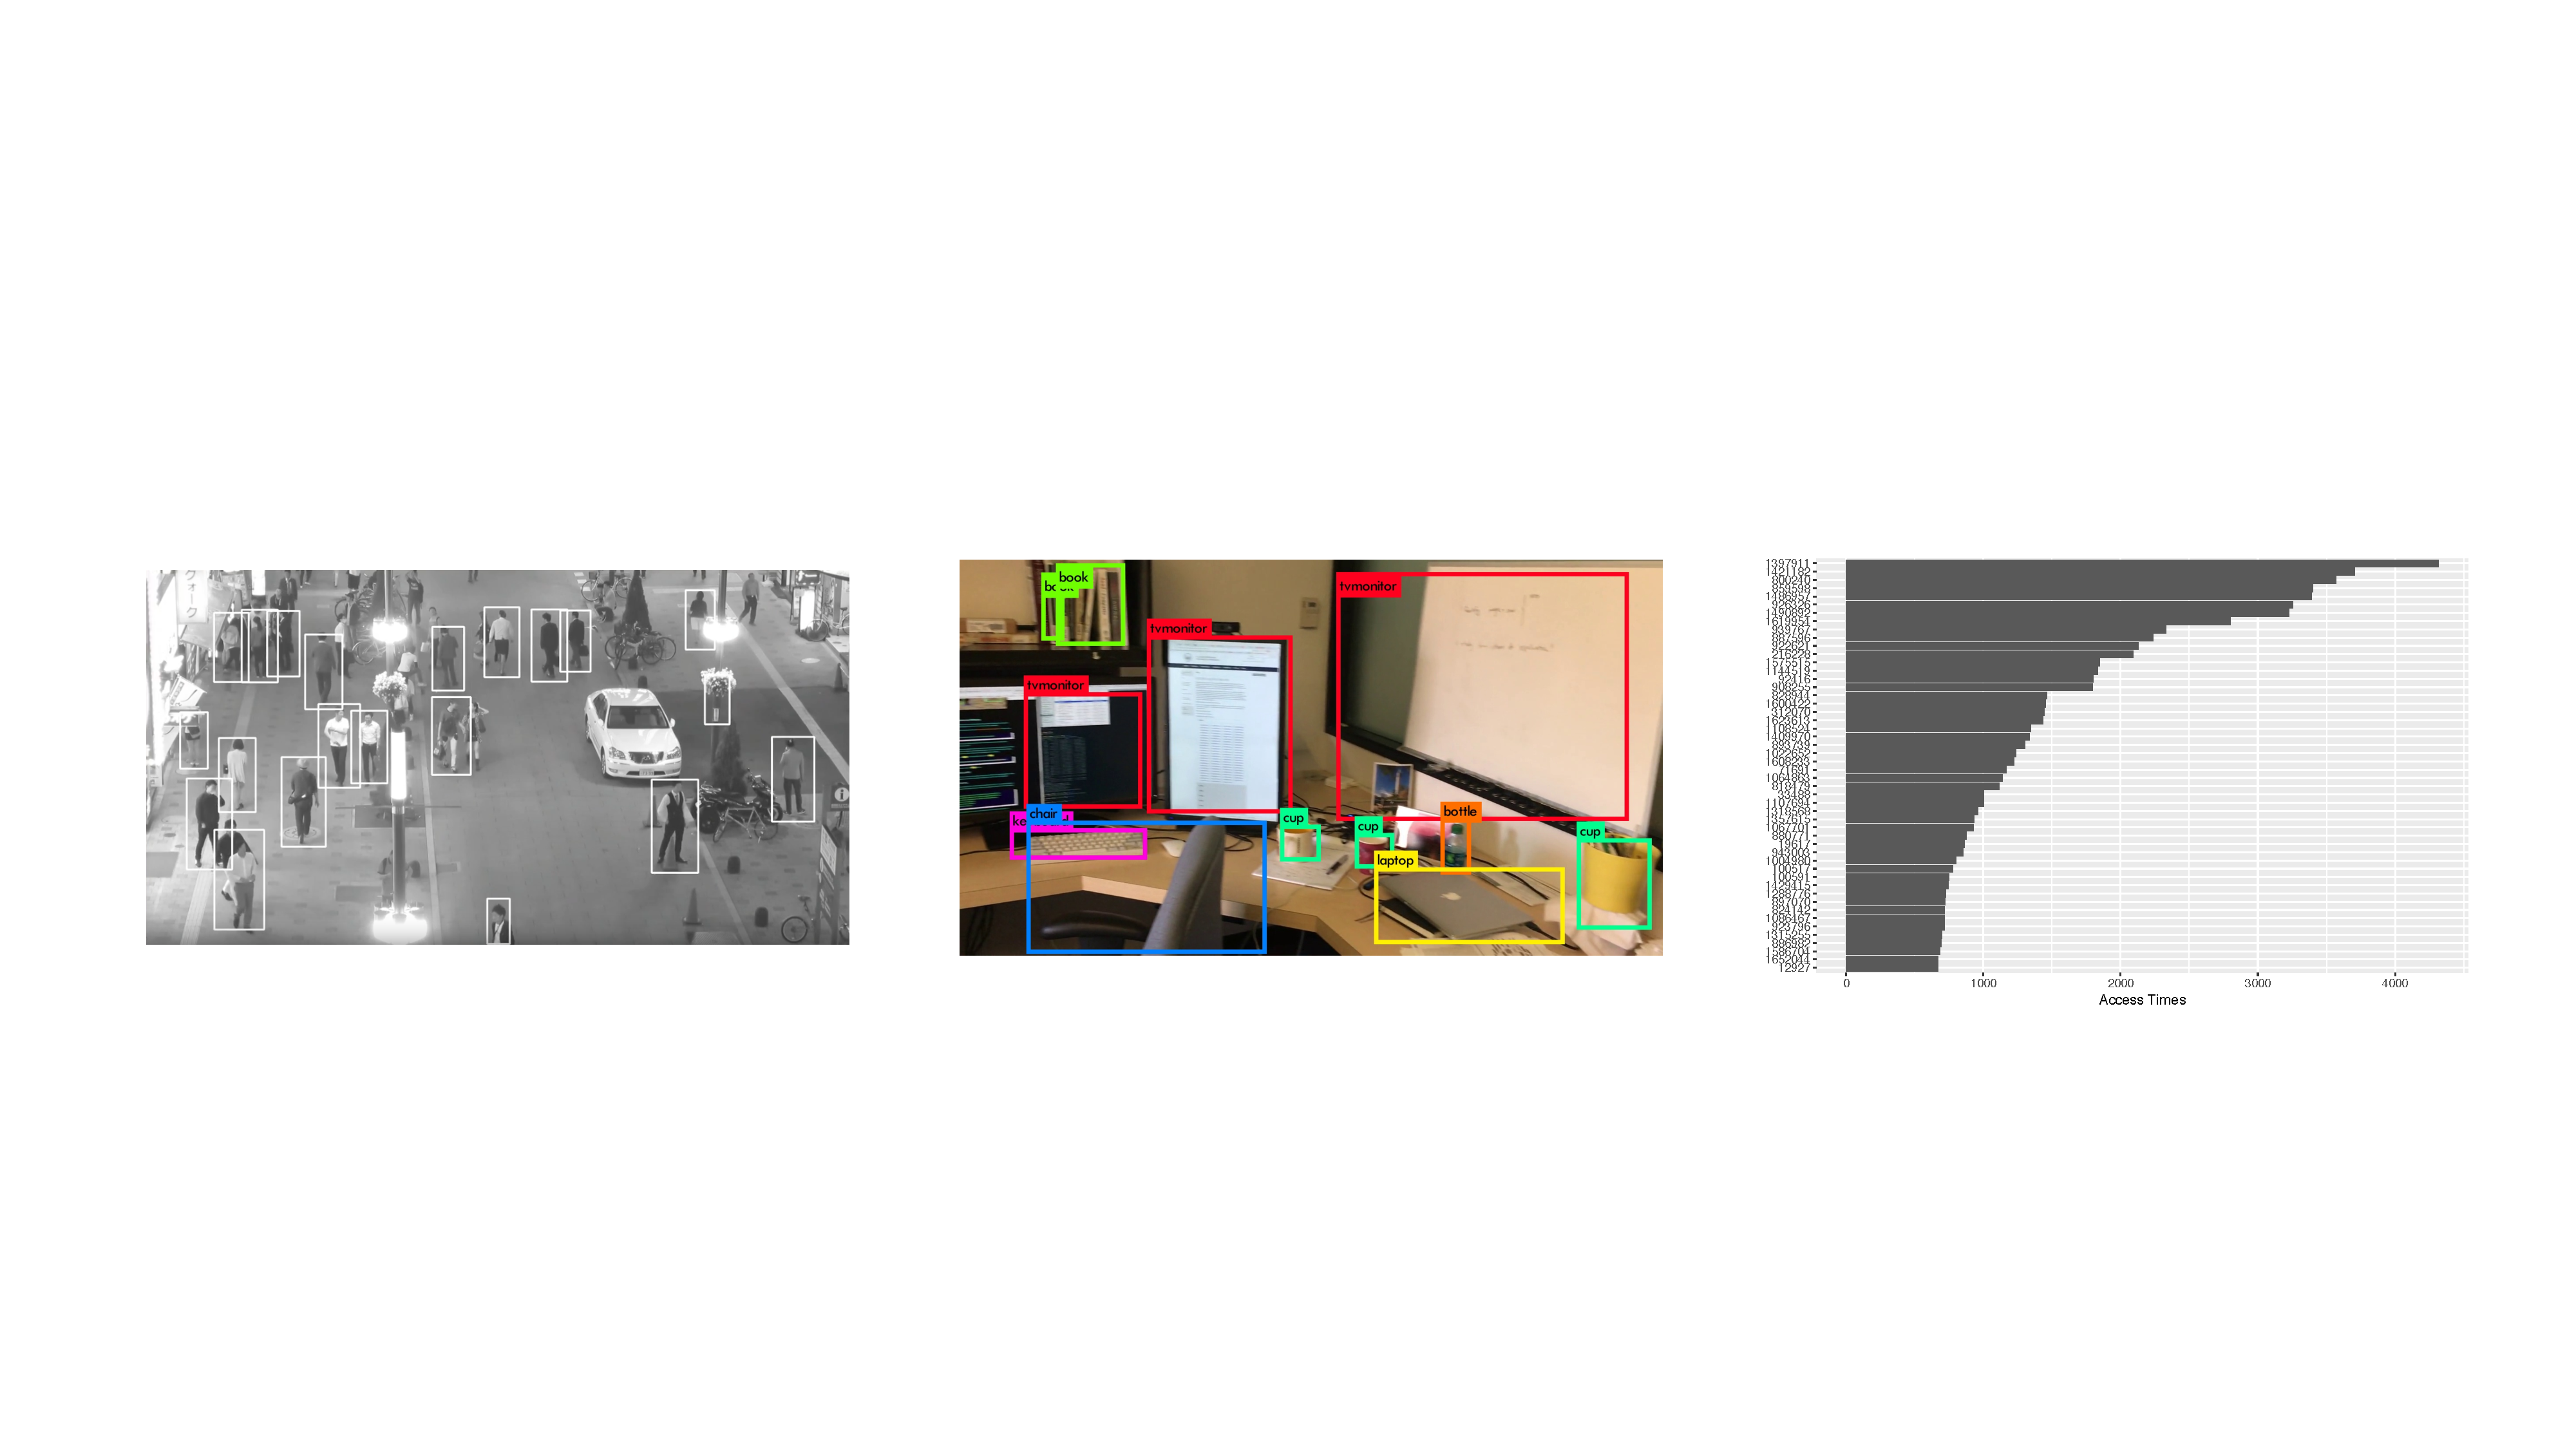
\includegraphics[width=\columnwidth]{figures/apps.pdf}
%   \caption{Three \sysname{} applications: augmented reality, pedestrian
%     detection, and distributed Top-K.}
%   \label{fig:three-apps}
% \end{figure}

\begin{table}
  \footnotesize
  \centering
  \begin{tabular}{c c c c}
    \toprule
    Application & Knobs & Accuracy & Dataset \\
    \midrule
    \specialcell{Augmented\\Reality}
                & \specialcell{resolution \\ frame rate \\ quantization }
                & F1 score~\cite{Rijsbergen:1979:IR:539927}
                & \specialcell{iPhone video clips\\training: office (24
    s)\\testing: home (246 s)} \\
    \midrule
    \specialcell{Pedestrian\\Detection}
                & \specialcell{resolution \\ frame rate \\ quantization }
                & F1 score
                & \specialcell{MOT16~\cite{milan2016mot16}\\training: MOT16-04\\testing: MOT16-03} \\
    \midrule
    \specialcell{Log Analysis\\(Top-K, K=50)}
                & \specialcell{head (N) \\ threshold (T) }
                & \specialcell{Kendall's $\tau$~\cite{abdi2007kendall}}
                & \specialcell{\href{https://www.sec.gov}{SEC.gov} logs~\cite{edgarlog} \\ training: 4 days \\
    testing: 16 days} \\
    \bottomrule
  \end{tabular}
  \caption{Application details.}
  \label{tab:apps}
  \vspace{-1em}
\end{table}

Using \sysname{}, we have built three applications: augmented reality (AR) that
recognizes nearby objects on mobile phones, pedestrian detection (PD) for
surveillance cameras, and a distributed log analysis to extract the Top-K mostly
accessed files (TK). \autoref{tab:apps} summarizes the application-specific
part: knobs, accuracy functions, and datasets.

\para{Augmented Reality.} We target at mobile augmented reality applications
that recognize objects by offloading the heavy computation elsewhere, e.g.\,the
cloud. We use OpenCV 3.1~\cite{opencvlibrary} for image-related operations and
YOLO~\cite{darknet13, redmon2016yolo9000}, a GPU-enabled pre-trained neural
network, for object recognition. Videos are encoded with
H.264~\cite{richardson2011h} because of its prevalence in existing systems. Our
implementation uses GStreamer~\cite{gstreamer} with \texttt{x264enc} plugin
(\texttt{zerolatency} and constant quality). The quantization factor is exposed
as a knob (in addition to image resolutions and frame rates).

Object recognition returns a list of bounding boxes with the type of the object,
and each bounding box is a rectangle with normalized coordinates on the
image. We compare the detection against the reference result from raw data, and
declare it success if the intersection over union (IOU) is greater than
50\%~\cite{everingham2010pascal} and the object type matches. We use F1
score~\cite{Rijsbergen:1979:IR:539927} as the accuracy function. In terms of
dataset, we collected our own video clips: the training data is a 24-second long
video of an office environment; the test data is a 246-second long video of a
home environment.

\para{Pedestrian Detection.} This application analyzes streams of videos from
installed CCTV cameras and detects pedestrians inside. We use a similar setup
(OpenCV and GStreamer) as our augmented reality application except for the
analytical function. To detect pedestrians, we use GPU-accelerated histogram of
oriented gradients (HOG)~\cite{dalal2005histograms} with the default linear SVM
classifier from OpenCV. Because we do not recognize individual pedestrians, a
successful detection in this case only requires matching the bounding box. Our
evaluation uses MOT16 dataset~\cite{milan2016mot16} for both profiling and
runtime.

\begin{figure}
  \centering
  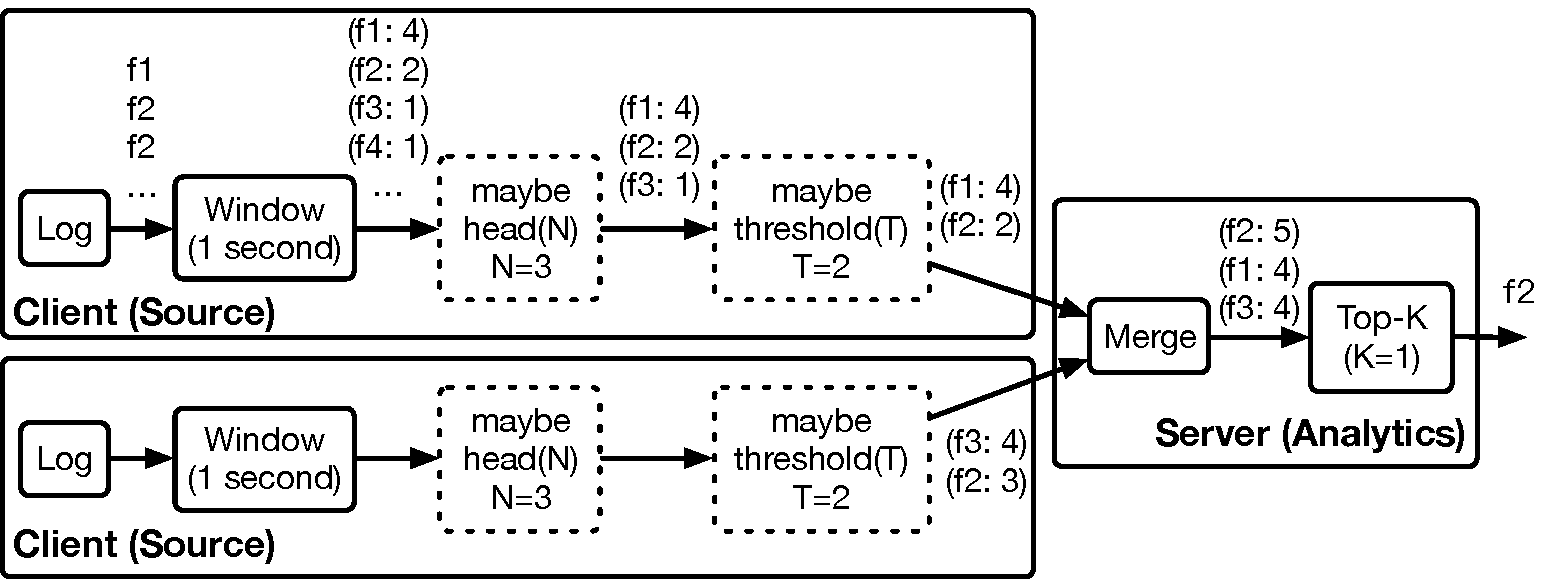
\includegraphics[width=\columnwidth]{figures/topk.pdf}
  \caption{A distributed Top-K application with two degradation operations:
    \texttt{head} and \texttt{threshold}. Discarding data with these two
    operations will affect final results. In this example, \texttt{f2}, which is
    not in Top-1 for either client, becomes the global Top-1 after the merge. It
    would have been purged if the clients use threshold T=3.}
  \label{fig:topk}
\end{figure}

\para{Distributed Top-K.} Many monitoring applications aggregate information
from geo-distributed servers to answer the \textit{Top-K}
question~\cite{babcock2003distributed}, such as the Top-K most popular URLs, or
the Top-K most access files. \autoref{fig:topk} shows our Top-K processing
pipeline with example data. Source nodes first summarizes the data with
\texttt{Window}. After the summary, the data size can still be too large because
most real-world access patterns follow a long tail distribution: there is a
large-but-irrelevant tail that contributes little to Top-K. The source nodes
perform two degradation operations: (1) a head(\texttt{N}) operation that only
takes the top \texttt{N} entries; (2) a threshold(\texttt{T}) that filters small
entries whose count is smaller than \texttt{T}. These two operations are not
orthogonal. Their impact on data size reduction and quality degradation depends
on the data distribution.

For accuracy, we use Kendall's~$\tau$~\cite{abdi2007kendall}, a correlation
measure of the concordance between two ranked list. The output ranges from
\(-1\) to 1, representing no agreement to complete agreement. To integrate with
\sysname{}, we convert Kendall's~$\tau$ to the range of [0, 1] with a linear
transformation. Our Top-K application aims to find the Top-50 most accessed
files from web server logs. We use Apache log files that record and store user
access statistics for the \href{https://www.sec.gov}{SEC.gov} website. The logs
are split into four groups, simulating four geo-distributed nodes monitoring web
accesses. To match the load of popular web servers, we compress one hour's logs
into one second.

%%% Local Variables:
%%% mode: latex
%%% TeX-master: "../awstream"
%%% End:
